%% =========================================================================
\section{Assistance Cognitive et Génération de Langage Naturel}
%% =========================================================================

Les moteurs de visualisation présentés dans la section précédente offrent à l'analyste une projection graphique du renseignement. Toutefois, l'interprétation de ces projections requiert une expertise contextuelle que les visualisations statiques ne peuvent fournir : face à un nœud CVE partagé entre deux acteurs APT, l'analyste doit déterminer la chaîne d'exploitation probable, évaluer la priorité de remédiation et formuler un plan d'action en langage naturel exploitable par les équipes opérationnelles. Nous avons implémenté un assistant cognitif conversationnel, baptisé \textbf{ONYX Copilot}, qui exploite un pipeline de \textit{Retrieval-Augmented Generation} (RAG) couplé au modèle de langage Gemini~2.0 Flash de Google pour fournir des réponses contextualisées, référencées et garanties sans hallucination.

\subsection{Architecture du Pipeline RAG}

Le pipeline RAG constitue le cœur du moteur d'assistance cognitive. Son architecture se décompose en quatre couches fonctionnelles : l'ingestion vectorielle, la recherche sémantique, l'augmentation contextuelle du prompt et la génération contrainte. Cette architecture est implémentée dans la classe \texttt{RAGPipeline} (module \texttt{rag\_pipeline.py}), orchestrée par le routeur FastAPI \texttt{chat.py} et consommée côté frontend par le composant \texttt{OnyxCopilot.tsx}.

\subsubsection{Couche 1 --- Ingestion et Vectorisation}

La première couche du pipeline transforme les documents CTI textuels en vecteurs numériques dans un espace de haute dimension. Les indicateurs de compromission armés (\textit{armed IOCs}), enrichis par le moteur de décroissance du chapitre précédent, sont convertis en documents textuels structurés via la méthode \texttt{seed\_from\_iocs()}. Chaque document encode le type d'indicateur, la valeur, la source OSINT, la sévérité, les étiquettes de classification et la famille de malware associée. Ces documents sont ensuite vectorisés par le modèle d'embeddings \texttt{gemini-embedding-2-preview} qui produit des vecteurs de dimension 3\,072, offrant une granularité sémantique suffisante pour distinguer des indicateurs thématiquement proches (par exemple, deux adresses IP appartenant à des infrastructures C2 distinctes).

Les vecteurs résultants sont indexés dans une collection Qdrant configurée avec la métrique de similarité \textit{cosinus}. Le service supporte deux modes d'infrastructure : un mode \textit{in-memory} pour le développement et la démonstration (latence nulle, persistance éphémère), et un mode distant connectant un cluster Qdrant de production via URL et clé API. Ce dualisme d'infrastructure garantit que le pipeline RAG fonctionne identiquement en environnement de développement local et en déploiement opérationnel.

\subsubsection{Couche 2 --- Recherche Sémantique}

Lorsqu'un analyste soumet une requête en langage naturel (par exemple : \og \textit{Quels sont les IOCs liés à Lazarus Group sur les dernières 24 heures ?} \fg{}), la requête est vectorisée par le même modèle d'embeddings, puis une recherche de similarité cosinus est effectuée dans la collection Qdrant pour extraire les \( k = 5 \) documents les plus pertinents (\textit{top-k retrieval}). Chaque résultat retourné comprend le contenu textuel du document, la source OSINT d'origine et un score de similarité compris entre 0 et 1.

\subsubsection{Couche 3 --- Augmentation Contextuelle et Prompt Engineering}

Les documents récupérés sont formatés en blocs de contexte numérotés et annotés avec leur source et leur score de pertinence, puis injectés dans un prompt structuré obéissant au patron suivant :

\begin{lstlisting}[language=Python, caption={Prompt système RAG avec politique de zéro-hallucination et contexte récupéré dynamiquement.}, label={lst:rag-prompt}]
RAG_SYSTEM_PROMPT = (
    "You are ONYX, a CTI Assistant.\n"
    "For factual queries regarding IPs, domains, "
    "or threats, strictly rely on retrieved context.\n"
    "If context is missing, state that you lack "
    "sufficient intelligence.\n"
    "Do not hallucinate IOCs or threat data.\n"
    "Format IOCs inside code blocks.\n"
    "Reference data source when available.\n"
    "Never provide exploit code or attack scripts.\n"
    "Use cold, analytical, surgical tone.\n\n"
    "RETRIEVED CONTEXT:\n{context}\n\n"
    "USER QUERY:\n{query}"
)
\end{lstlisting}

Ce prompt implémente une politique de \textbf{zéro-hallucination} via six contraintes explicites : (1)~l'obligation de s'appuyer exclusivement sur le contexte récupéré pour toute assertion factuelle, (2)~l'aveu explicite d'insuffisance d'intelligence en cas de contexte manquant, (3)~l'interdiction de fabriquer des indicateurs non présents dans le contexte, (4)~le formatage systématique des IOC en blocs de code pour la lisibilité, (5)~la référence obligatoire aux sources, et (6)~l'interdiction de générer du code offensif. Cette approche diffère fondamentalement d'un chatbot généraliste : le modèle ne peut répondre qu'à partir de données vérifiées et indexées dans le magasin vectoriel.

\subsubsection{Couche 4 --- Génération Contrainte et Streaming SSE}

La génération est effectuée par le modèle Gemini~2.0~Flash via le SDK Google GenAI. Le service \texttt{GeminiService} implémente un mécanisme de résilience par \textit{exponential backoff with full jitter} (backoff exponentiel avec gigue complète, style AWS) sur les codes de retour 429 (\textit{rate limit}) et 503 (\textit{service unavailable}), avec un maximum de 5~tentatives et un délai plafonné à 60~secondes. Ce mécanisme distingue les erreurs de quota strictes (épuisement du compte de facturation) des limitations de débit transitoires, levant une exception \texttt{QuotaExhaustedException} dans le premier cas et ré-essayant silencieusement dans le second.

Le flux de réponse est transmis au frontend via \textit{Server-Sent Events} (SSE) conformément au protocole compatible \texttt{deep-chat}. Chaque chunk de texte généré est encapsulé dans un événement SSE au format \texttt{data: \{"text": "..."\}}, permettant un affichage progressif en temps réel dans l'interface conversationnelle. Le flux est terminé par un événement sentinelle \texttt{data: [DONE]}.

\subsection{Sécurisation par Garde-fous (\textit{Guardrails})}

Le pipeline conversationnel est protégé par un moteur de garde-fous bidirectionnel, le \texttt{GuardrailsEngine}, inspiré de l'architecture NeMo Guardrails de NVIDIA. Ce moteur opère en validation \textit{pré-génération} (sur l'entrée utilisateur) et \textit{post-génération} (sur la sortie du modèle), implémentant un filtrage symétrique.

\begin{table}[H]
\centering
\caption{Garde-fous de sécurité du pipeline conversationnel : règles de validation entrée/sortie.}
\label{tab:guardrails}
\begin{tabular}{|l|l|l|l|}
\hline
\textbf{Direction} & \textbf{Type de Violation} & \textbf{Mécanisme} & \textbf{Action} \\
\hline
Entrée & Injection de prompt & Regex compilés (YAML) & HTTP 403 \\
\hline
Entrée & Jailbreak & Regex compilés (YAML) & HTTP 403 \\
\hline
Entrée & Sujet hors périmètre CTI & Vérification mots-clés CTI & HTTP 403 \\
\hline
Entrée & Longueur excessive & Plafond 4\,000 caractères & HTTP 403 \\
\hline
Sortie & Fuite de PII & Regex (SSN, email, etc.) & Suppression \\
\hline
Sortie & Fuite de credentials & Regex (API keys, tokens) & Suppression \\
\hline
Sortie & Contenu toxique & Regex compilés & Suppression \\
\hline
Sortie & Longueur excessive & Plafond 16\,000 caractères & Troncature \\
\hline
\end{tabular}
\end{table}

Les règles sont déclarées dans un fichier YAML externe (\texttt{guardrails\_config.yml}), chargé et compilé paresseusement (\textit{lazy loading}) au premier appel. Cette séparation entre la logique de validation et la configuration des règles permet à l'équipe SOC de mettre à jour les patrons de détection sans modifier le code source du service.

\subsection{Interface Conversationnelle Frontend}

Le composant \texttt{OnyxCopilot} est injecté globalement dans le \texttt{RootLayout} Next.js via un import dynamique SSR-safe (\texttt{dynamic(() => import(...), \{ssr: false\})}). Il se manifeste sous forme d'un bouton d'action flottant (\textit{Floating Action Button}) positionné en bas à droite de l'écran, accessible depuis toute vue de la plateforme. L'ouverture déclenche une animation \textit{slide-up} avec courbe d'accélération cubique-bézier.

La fenêtre conversationnelle gère trois types de messages visuellement distincts : les réponses normales rendues par le composant \texttt{TerminalMessage} avec mise en forme Markdown et blocs de code syntaxiquement colorés, les alertes de garde-fou (\textit{guardrail blocks}) affichées avec un encadrement rouge et une icône de bouclier, et les alertes de quota affichées en orange avec un indicateur pulsant. L'état de session est maintenu par un identifiant \texttt{session\_id} transmis via l'en-tête HTTP \texttt{X-Session-Id}, permettant la continuité conversationnelle sur 20~messages d'historique.

\begin{figure}[H]
    \centering
    \makebox[\textwidth][c]{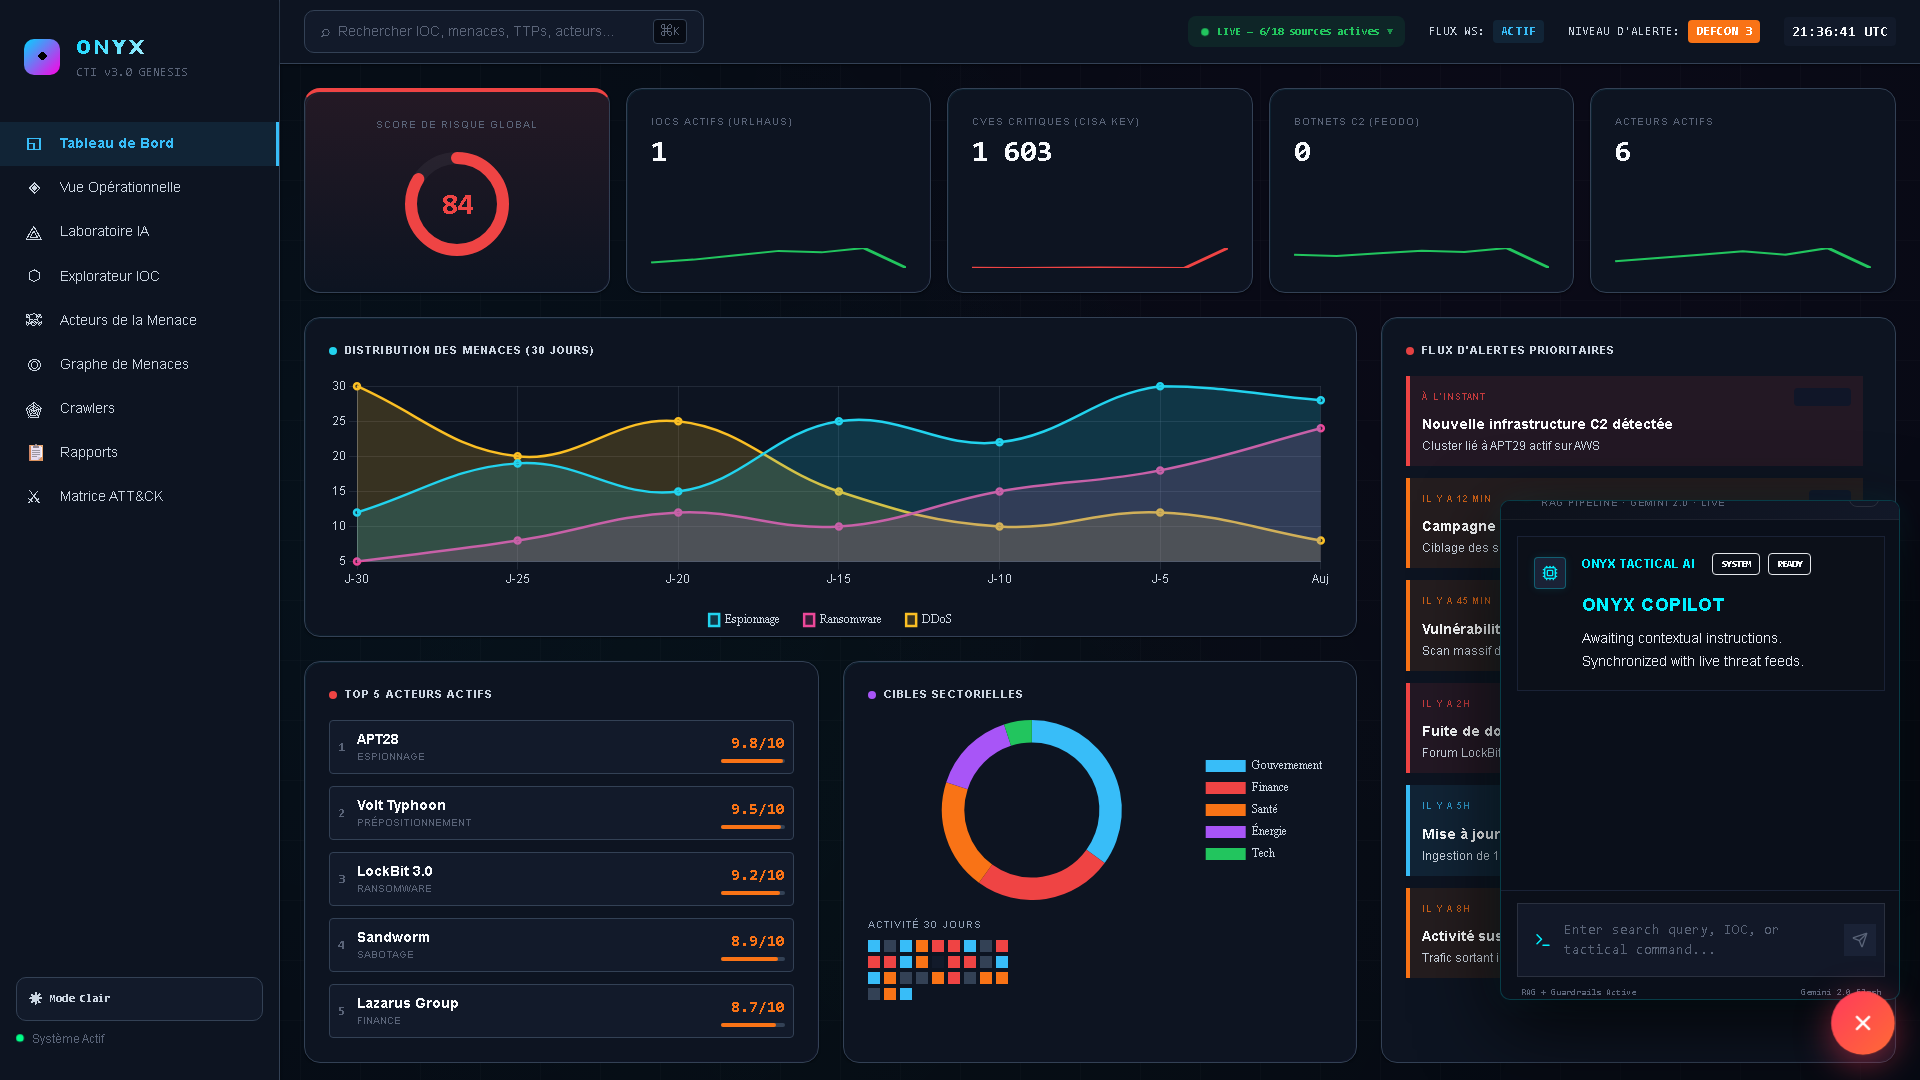
\includegraphics[width=1.0\textwidth, keepaspectratio]{assistant_chatbot.png}}
    \caption{Interface de l'assistant ONYX Copilot : fenêtre conversationnelle flottante avec pipeline RAG, streaming SSE et indicateur d'état « RAG + Guardrails Active ». Le modèle sous-jacent est Gemini~2.0~Flash.}
    \label{fig:assistant_chatbot}
\end{figure}

La figure~\ref{fig:assistant_chatbot} illustre l'interface conversationnelle en conditions opérationnelles. Nous observons le message de bienvenue système (indicateur \texttt{SYSTEM | READY}), la zone de saisie de commandes avec les indicateurs de statut du pipeline (RAG et Guardrails actifs) et le bouton d'action flottant.

%% =========================================================================
\section{Interopérabilité et Exportation Opérationnelle}
%% =========================================================================

Le renseignement sur les cybermenaces n'acquiert de valeur opérationnelle que lorsqu'il est traduit en artefacts directement exploitables par les systèmes de défense. Un rapport d'analyse non intégré dans les pare-feux, les EDR et les SIEM reste un document d'intérêt académique. Nous avons implémenté trois vecteurs d'exportation opérationnelle dans la plateforme ONYX : la génération automatisée de règles de détection (YARA, Sigma, Snort), l'exportation de rapports PDF structurés et la production de bundles STIX~2.1 interopérables.

\subsection{Génération Automatisée de Règles de Détection}

Le composant \texttt{SIEMRuleConverter} implémente un compilateur de règles de détection qui transforme les indicateurs de compromission armés par le \textit{Decay Engine} en signatures opérationnelles pour trois moteurs de détection distincts.

\subsubsection{Règles Sigma}

Le format Sigma, développé par Florian Roth, constitue un standard ouvert de description de signatures SIEM agnostique vis-à-vis du produit commercial. Le compilateur ONYX génère des règles Sigma en YAML avec les champs suivants : un identifiant UUID unique (\texttt{id}), un statut \texttt{production}, une description incluant l'adresse IP cible et la source OSINT, une source de logs de type \texttt{network\_connection} pour le produit Zeek, une clause de détection avec sélection par IP cible et exclusion des plages RFC~1918, des faux positifs documentés, un niveau de criticité \texttt{critical}, et des tags MITRE ATT\&CK (\texttt{T1071.001}, \texttt{T1095}). Le compilateur applique automatiquement un filtre d'exclusion des plages internes (\texttt{10.*}, \texttt{192.168.*}) pour réduire les faux positifs.

\subsubsection{Règles YARA}

Les règles YARA sont compilées avec une structure multi-chaînes optimisée pour la détection en mémoire et sur disque. Chaque règle inclut quatre chaînes de correspondance : l'adresse IP en encodage ASCII (\texttt{ascii wide nocase}), l'adresse IP en encodage hexadécimal (pour la détection dans les flux binaires), un marqueur d'agent utilisateur automatisé (\texttt{python-requests}), et une séquence d'octets caractéristique d'un appel de beacon C2 (\texttt{48 8B ?? E8 ?? ?? ?? ?? 48 85 C0}). La clause de condition est formulée comme une disjonction logique : la présence de l'un des patrons IP \textbf{ou} la conjonction du patron d'appel de beacon et du marqueur d'agent utilisateur. Cette formulation maximise le rappel tout en maintenant la précision par la spécificité de la séquence hexadécimale.

\subsubsection{Règles Snort}

Les signatures Snort sont générées au format IDS/IPS avec les métadonnées opérationnelles complètes : type de classification (\texttt{trojan-activity}), identifiant de signature unique calculé par hachage déterministe de l'adresse IP cible, périmètre de déploiement (\texttt{Perimeter}), gravité (\texttt{Critical}) et tag de catégorisation (\texttt{C2}).

\subsubsection{Rotation Automatique et Alimentation Live}

Le compilateur opère en mode continu : les IOC armés sont extraits du store Zustand (\texttt{armedIocs}), filtrés par type IPv4 et par seuil de confiance ($\geq 90\%$), et injectés dans les templates de règles avec une rotation automatique toutes les 5~secondes. Ce mécanisme garantit que l'analyste dispose en permanence de règles pré-compilées pour les IOC les plus récents et les plus fiables, directement copiables dans son environnement SIEM via le bouton d'export en un clic.

\subsection{Exportation de Rapports PDF Structurés}

Le composant \texttt{ReportGenerator} implémente un moteur de génération de rapports PDF exploitant la bibliothèque \texttt{jsPDF} pour le rendu côté client. L'architecture du rapport suit une structure normalisée en quatre sections obligatoires :

\begin{enumerate}
    \item \textbf{Page de couverture} : fond slate-900, encadrement TLP chromatiquement codé (rouge, ambre ou vert), identifiants de classification (\texttt{TLP:RED}, \texttt{TLP:AMBER}, \texttt{TLP:GREEN}), date de génération, auteur et référence unique.
    \item \textbf{Synthèse exécutive (BLUF)} : cinq points de renseignement structurés selon la doctrine militaire \textit{Bottom Line Up Front} --- niveau de menace, acteur principal, surface d'exposition, vecteurs d'attaque et risque métier --- suivis d'un plan d'action immédiat en trois volets (isolation, blocage, révocation).
    \item \textbf{Fiches thématiques par acteur} : pour chaque acteur de menace identifié (maximum 5), une fiche complète incluant le profil de menace (alias, origine, motivation, cibles, sévérité), le modus operandi (TTPs MITRE ATT\&CK et arsenal), et un tableau d'IOC majeurs avec type, source et sévérité.
    \item \textbf{Matrice de remédiation technique} : actions défensives catégorisées par domaine d'infrastructure (Réseau \& Périmètre, Identité \& Accès, Endpoints) avec commandes exécutables et justifications.
\end{enumerate}

Le rapport est conditionné par le niveau de classification TLP sélectionné par l'analyste. Le niveau \texttt{TLP:RED} (\textit{Technique \& Urgent}) produit un rapport complet de 4 à 6 pages incluant tous les indicateurs techniques. Le niveau \texttt{TLP:AMBER} (\textit{Opérationnel}) produit un rapport tactique de 4 à 5 pages avec IOC filtrés. Le niveau \texttt{TLP:GREEN} (\textit{Exécutif}) produit un rapport stratégique de 3 à 4 pages concentré sur la synthèse et les TTPs.

\subsection{Exportation STIX 2.1 Interopérable}

Le second vecteur d'exportation produit un bundle JSON conforme au standard OASIS STIX~2.1, permettant l'interopérabilité avec les plateformes MISP, OpenCTI, TheHive et toute plateforme supportant le protocole TAXII. Le pipeline d'exportation opère en trois étapes : (1)~récupération des acteurs de menace et des IOC armés via les endpoints REST du backend, (2)~déduplication stricte des IOC par valeur via une structure \texttt{Map} JavaScript éliminant les doublons issus de sources OSINT multiples, et (3)~transformation en objets STIX typés (\texttt{threat-actor}, \texttt{indicator}) avec identifiants UUID et horodatage conformes au schéma STIX~2.1. Chaque indicateur est encodé avec un patron STIX valide (ex. : \texttt{[ipv4-addr:value = '185.220.101.47']}).

\begin{figure}[H]
    \centering
    \makebox[\textwidth][c]{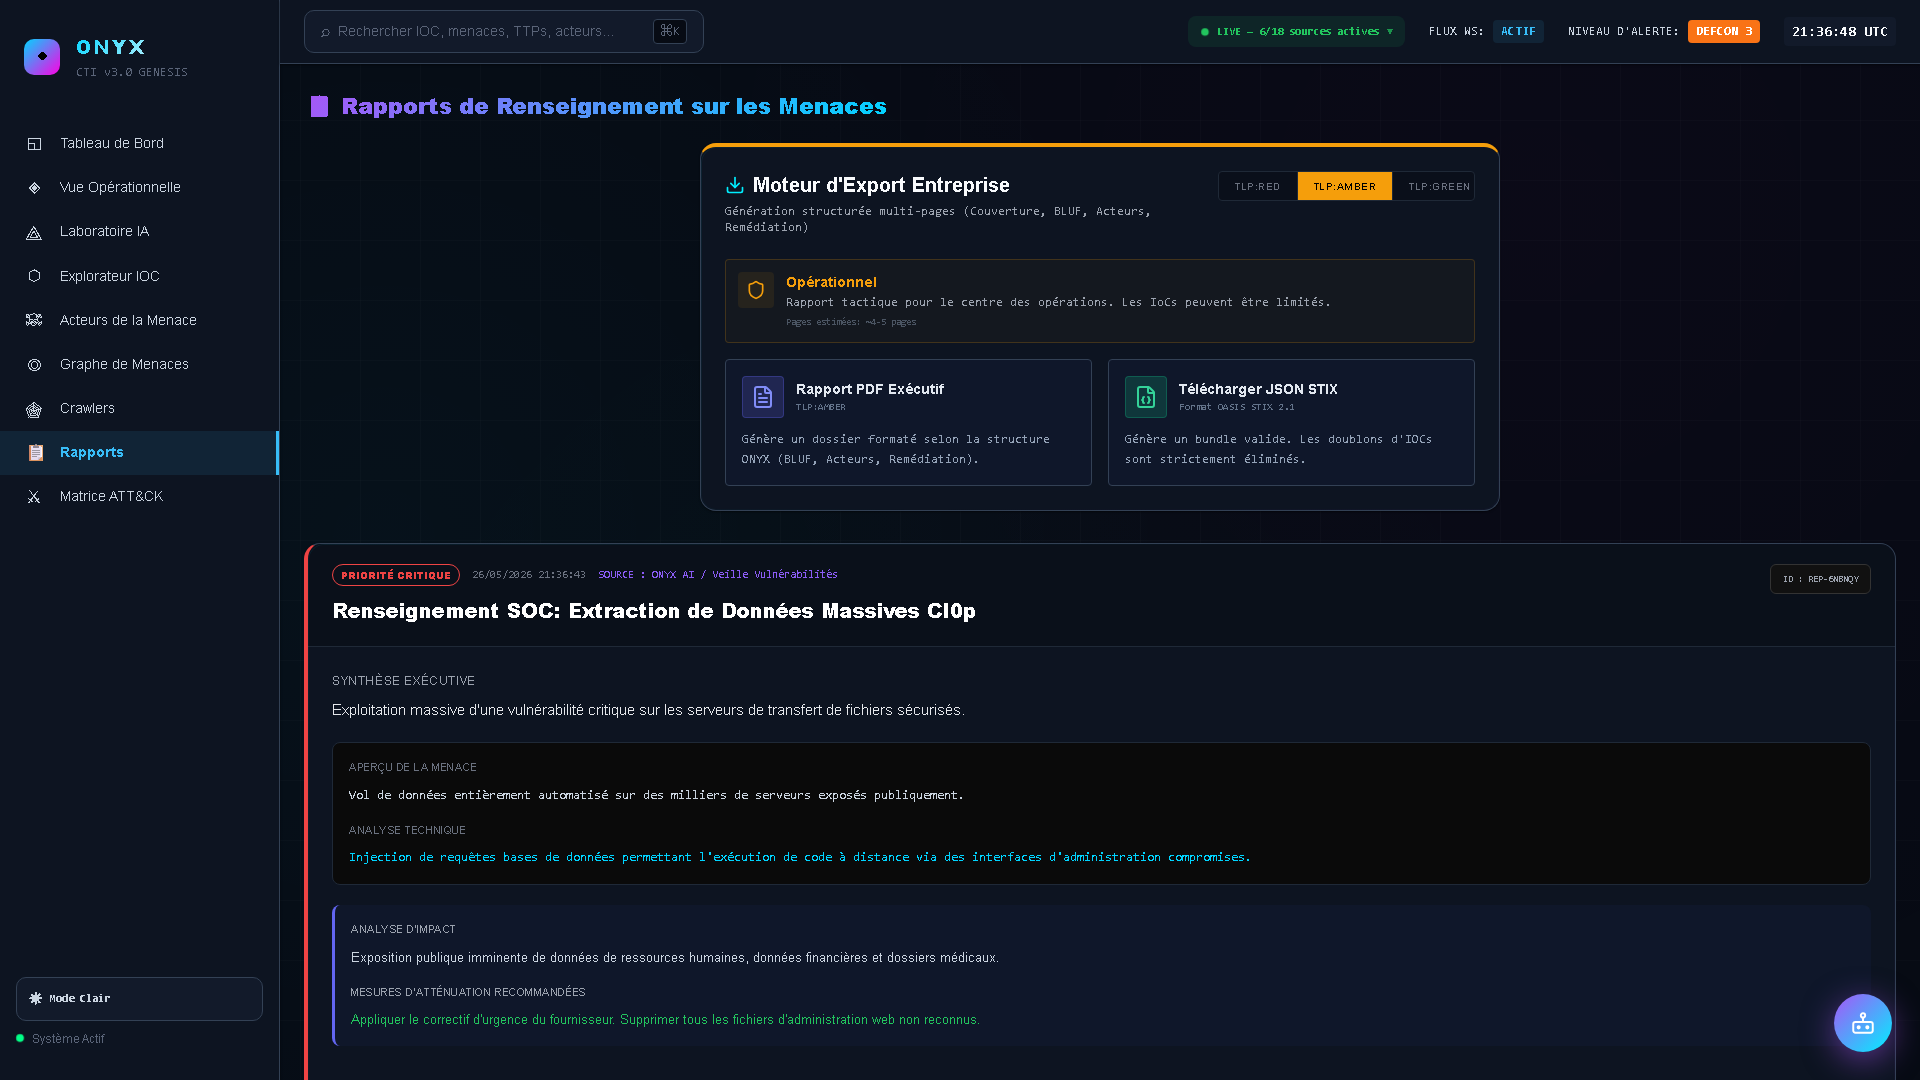
\includegraphics[width=1.0\textwidth, keepaspectratio]{export_rules.png}}
    \caption{Module d'exportation opérationnelle : générateur de rapports PDF multi-TLP (couverture, BLUF, fiches acteurs, matrice de remédiation), export STIX~2.1 et moteur d'ingénierie de détection (YARA/Sigma/Snort) avec alimentation OSINT en temps réel.}
    \label{fig:export_rules}
\end{figure}

La figure~\ref{fig:export_rules} présente le module d'exportation en conditions opérationnelles. Nous observons le sélecteur de classification TLP, les boutons d'export PDF et STIX~2.1, le visualiseur de bundle STIX et le panneau d'ingénierie de détection avec les onglets Sigma, YARA et Snort affichant la règle compilée pour l'IOC courant extrait du flux OSINT en direct.
